One method of machine learning, although not mainly used for dimensional reduction, that takes into account a given classification are Decision Trees (there are some researchers that have studied the feature selection using them as \cite{sugumaran2007feature} and \cite{cho2011decision}). A Decision Tree \citep{rokach2008data} is a prediction model which, given a set of data, makes logical construction diagrams, very similar to rule-based prediction systems. These diagrams serve to represent and categorize a series of conditions that occur successively for the resolution of a problem. There are many algorithms to implement them. We are going to use an optimised version of the CART algorithm \citep{breiman1984classification} with entropy as its criterion.

The advantages of Decision Trees are that they take into account the defined categorisation, as it is a supervised machine learning classification method, and that they are very explainable. However, our purpose is to know the features that best describe the writing style based on the recipient, instead of classifying new messages. For this reason, we are going to make use of the structure of the constructed Decision Tree in order to measure the importance that each style metric has in it.

\begin{figure}[h]
	\centering%
	\centerline{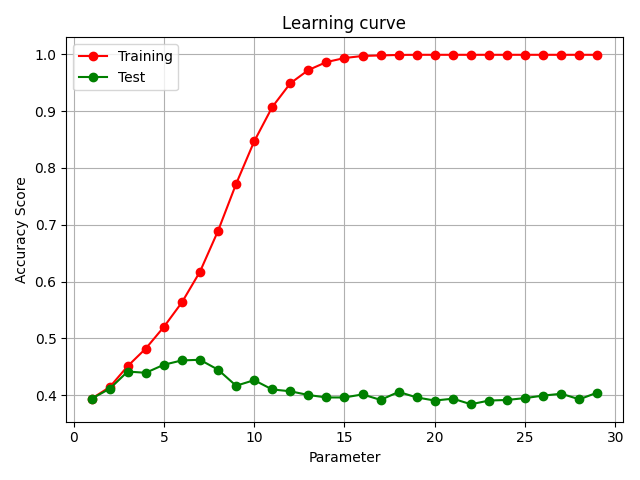
\includegraphics[width=0.7\textwidth]{Imagenes/Bitmap/DecisionTrees/learning28curve.png}}%
	\caption{Learning curve with the 28 chosen features}%
	\label{fig:learn28curve}
\end{figure}

A good intuition is to think that, in order to study the importance of a node, it is important to bear its depth in the tree in mind, because the lower it is, the more elements it differentiates. However, it will not be so useful if it just separates elements of the same class. Likewise, the number of samples that reach the node and its category is an important factor to keep in mind. Nevertheless, it will not be helpful if it maintains the proportion of each category in its child nodes. We are able to think of many parameters that can have relevance in the definition of the importance of a node in the Decision Tree. In this case we are going to use the Gini Importance \citep{breiman2001random}, which is defined by the following expression:

$$
ni_j = w_jH_j - w_{left(j)}H_{left(j)} - w_{right(j)}H_{right(j)}
$$

Where $ni_j$ is the importance of node j, $w_j$ is the weighted number of samples reaching node j, $H_j$ is the entropy of node j, $left(j)$ is the child node from left split on node j and $right(j)$ is the child node from right split on node j. Consequently, the importance of each feature is defined by the following formula:

$$
fi_i = \frac{\sum_{j\in Nod(i)}ni_j}{\sum_{j\in Nod}ni_j}
$$

Where $fi_i$ is the importance of feature i, $Nod(i)$ is the set of nodes which split on feature i and $Nod$ is the set of all nodes. In our study we are going to use the normalised feature importance, which is defined by the following expression:

$$
nfi_i=\frac{fi_i}{\sum_{j\in F}fi_j}
$$

\begin{figure}[t]
	\centering%
	\centerline{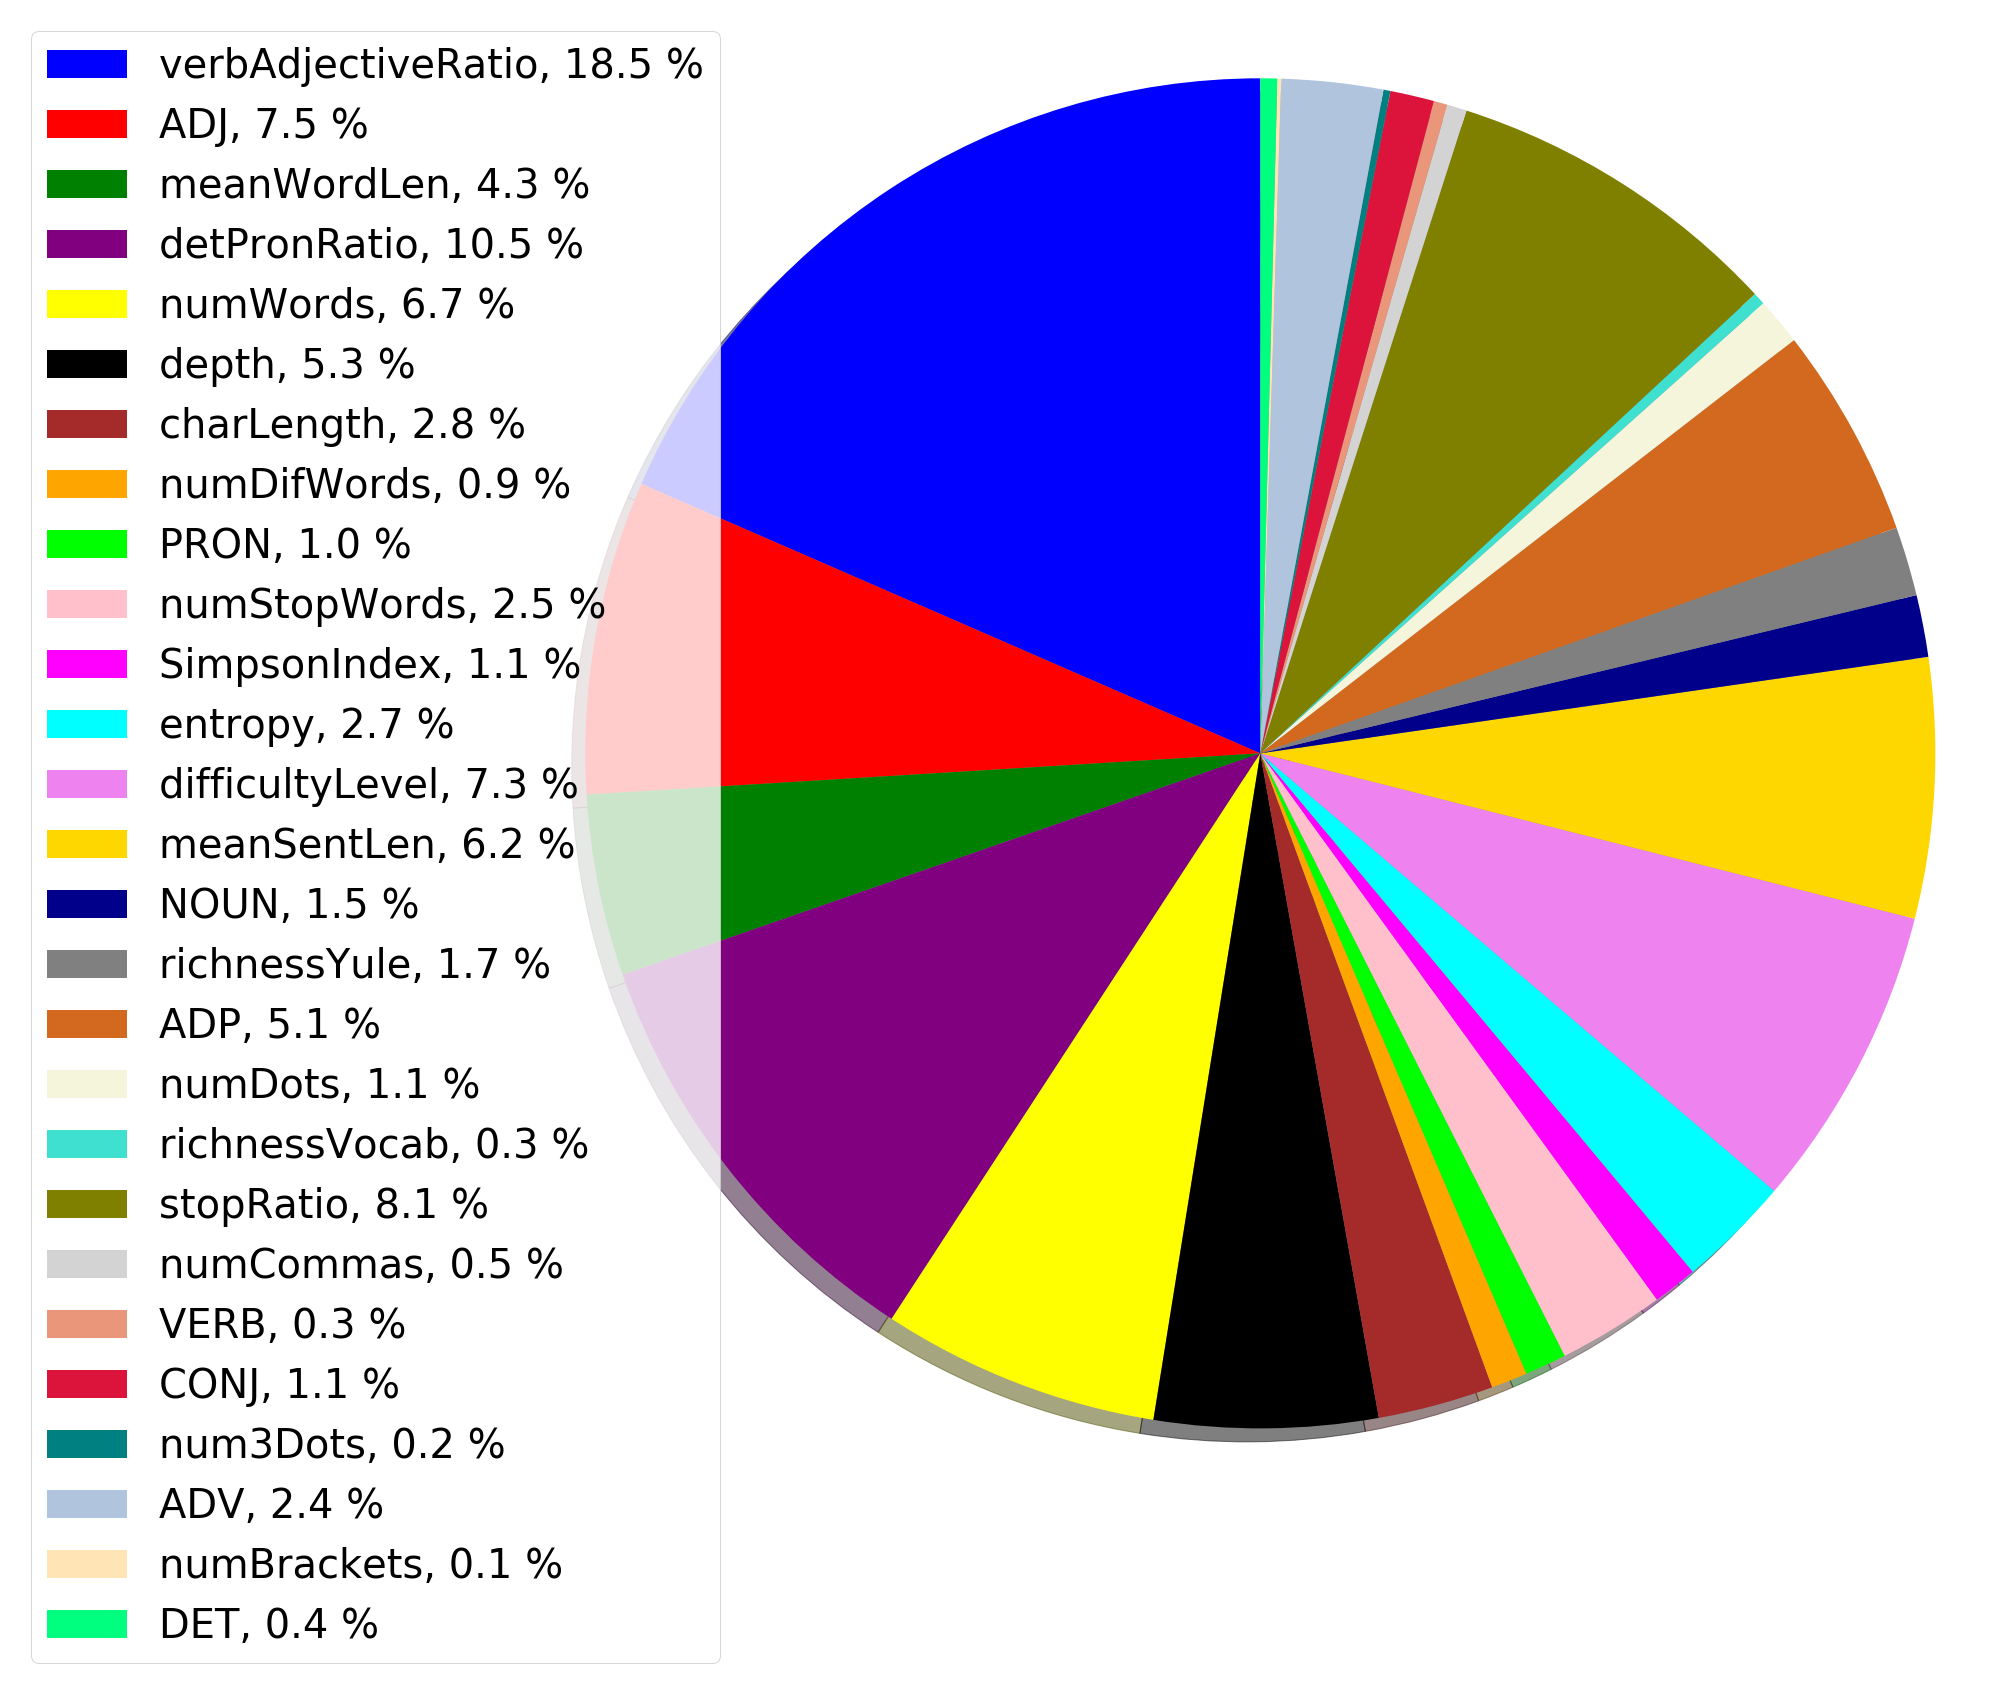
\includegraphics[width=0.8\textwidth]{Imagenes/Bitmap/DecisionTrees/pie28.png}}%
	\caption{Distribution of normalised feature importance with 28 features}%
	\label{fig:nfi28}
\end{figure}

Where $nfi_i$ is the normalised feature importance and $F$ is the set of features. Once we have the expression required for the analysis of the importance of each feature, we are able to calculate the distribution of the importance of each style metric with our 28 chosen style markers. To build the Decision Tree, we have to decide the depth of it. To take this decision, we calculate the learning curve both in training set and test set, and obtain the curves that we can observe in Figure \ref{fig:learn28curve} (the normalised data was used for the calculation of learning curve, as well as in the construction of the Decision Tree). Thus, we will choose a depth that avoids the overlearning (which could be produced in values of depth with which the training accuracy score is 1) and the missing of information (depth with which the training accuracy score is less than 0.9). Our choice will be the depth whose training accuracy score is the interval $(0.9, 1)$ and its test accuracy score is maximum (in this case it is eleven, but later, when we had less features, it will follow this criteria).

Making use of the explained expressions for the calculation of the normalised feature importance, we can go through the created tree with the chosen depth in order to obtain the distribution of this value. The result is shown in Figure \ref{fig:nfi28}.

As we can observe, the \textit{numSemiColon} characteristic does not appear in Figure \ref{fig:nfi28}, which means it has no importance in our constructed tree. Besides, \textit{verbAdjectiveRatio}, \textit{detPronRatio} and \textit{stopRatio} have the highest importance ratio and their related metrics (\textit{ADJ} and \textit{VERB}, \textit{DET} and \textit{PRON}, and \textit{numStopWords}, respectively) have a very small value. For this reason, we are able to claim that we can dispense with the related style features and \textit{numSemiColon} in order to describe the writing style. Therefore, we can construct another Decision Tree (by automatically taking a depth, as we have explained before) to calculate the importance ratio of each of the non-removed style markers. When we have the distribution of Gini Importance, we can remove again the non-important style metrics and those that have an extremely low importance ratio. By repeating this process, we are able to choose a small number of features which have a big importance ratio in the classification of the messages based on their recipients.

The learning curves of these iteration are all very similar to the one shown in Figure \ref{fig:learn28curve}. However, the evolution of the importance ratio of the style metrics is not uniform during all this iterative process. This behaviour could be seen in Figure \ref{fig:impcurv}.

\begin{figure}
	\centering%
	\centerline{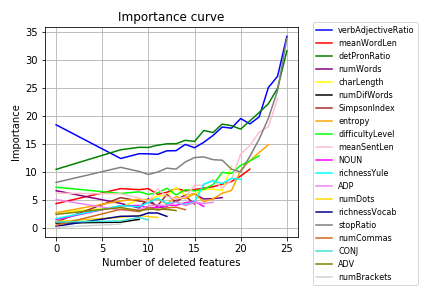
\includegraphics[width=0.9\textwidth]{Imagenes/Bitmap/DecisionTrees/limportancecurve.png}}%
	\caption{Evolution of importance ratio}%
	\label{fig:impcurv}
\end{figure}

Figure \ref{fig:impcurv} represents the importance ratio of each feature until it was removed from the set of style markers. The features that does not appear in the legend are those that were non-important in the first or second iteration, or were removed (such as the previously mentioned \textit{ADJ} and \textit{VERB}) before the second step.

Before detailing the different importance curves of each feature, there are some interesting general observations. Until the elimination of twenty features, which means having eight style metrics, it is always decided to dispense with some style marker whose importance is around 5\% compared to others that are above 10\%. From this point on, we see that characteristics with a more relevant importance start to be lost. From this fact we can deduce that keeping eight style metrics is a good principle to describe the style based on the recipient.

In general, the behaviour of most of the features is constant. As we can observe, most of the last eight style markers were the most important features at the beginning of the process. Of course, little by little, some of the metrics experience an increase due to, as the sum of all the non-removed metrics importance is always the same, the ratio has to be distributed between a lower number of characteristics. However, this increase becomes remarkable as soon as a big amount of style markers has been deleted (approximately from 20 removed features).

Thanks to the constant evolution of the importance of each metric, we can claim that most of the selected features (those which had not been removed until the number twenty), were those which had the highest values at the beginning; as well as, almost all of the deleted style markers when they have insignificant values of the ratio, were unimportant at the beginning. This fact allows us to assert that, given our dataset, our classification and our selected features, to add unimportant style markers does not excessively contribute to hide the really significant style descriptors.

Another possible assessment of the evolution of importance described by the Figure \ref{fig:impcurv} is that most of the features that are eliminated below 5\% of importance, before being so experience a slight decrease.

Going into more detail, the last eight selected features are: \textit{verbAdjectiveRatio}, \textit{detPronRatio}, \textit{meanSentLen}, \textit{meanWordLen}, \textit{richnessYule}, \textit{difficultyLevel}, \textit{stopRatio} and \textit{entropy}. All of them have an importance bigger than 8\% as we can see in the importance distribution of the Figure \ref{fig:nfi8}. Moreover, as we can check with Figure \ref{fig:correlation}, none of these metrics are directly correlated with each other.

\begin{figure}
	\centering%
	\centerline{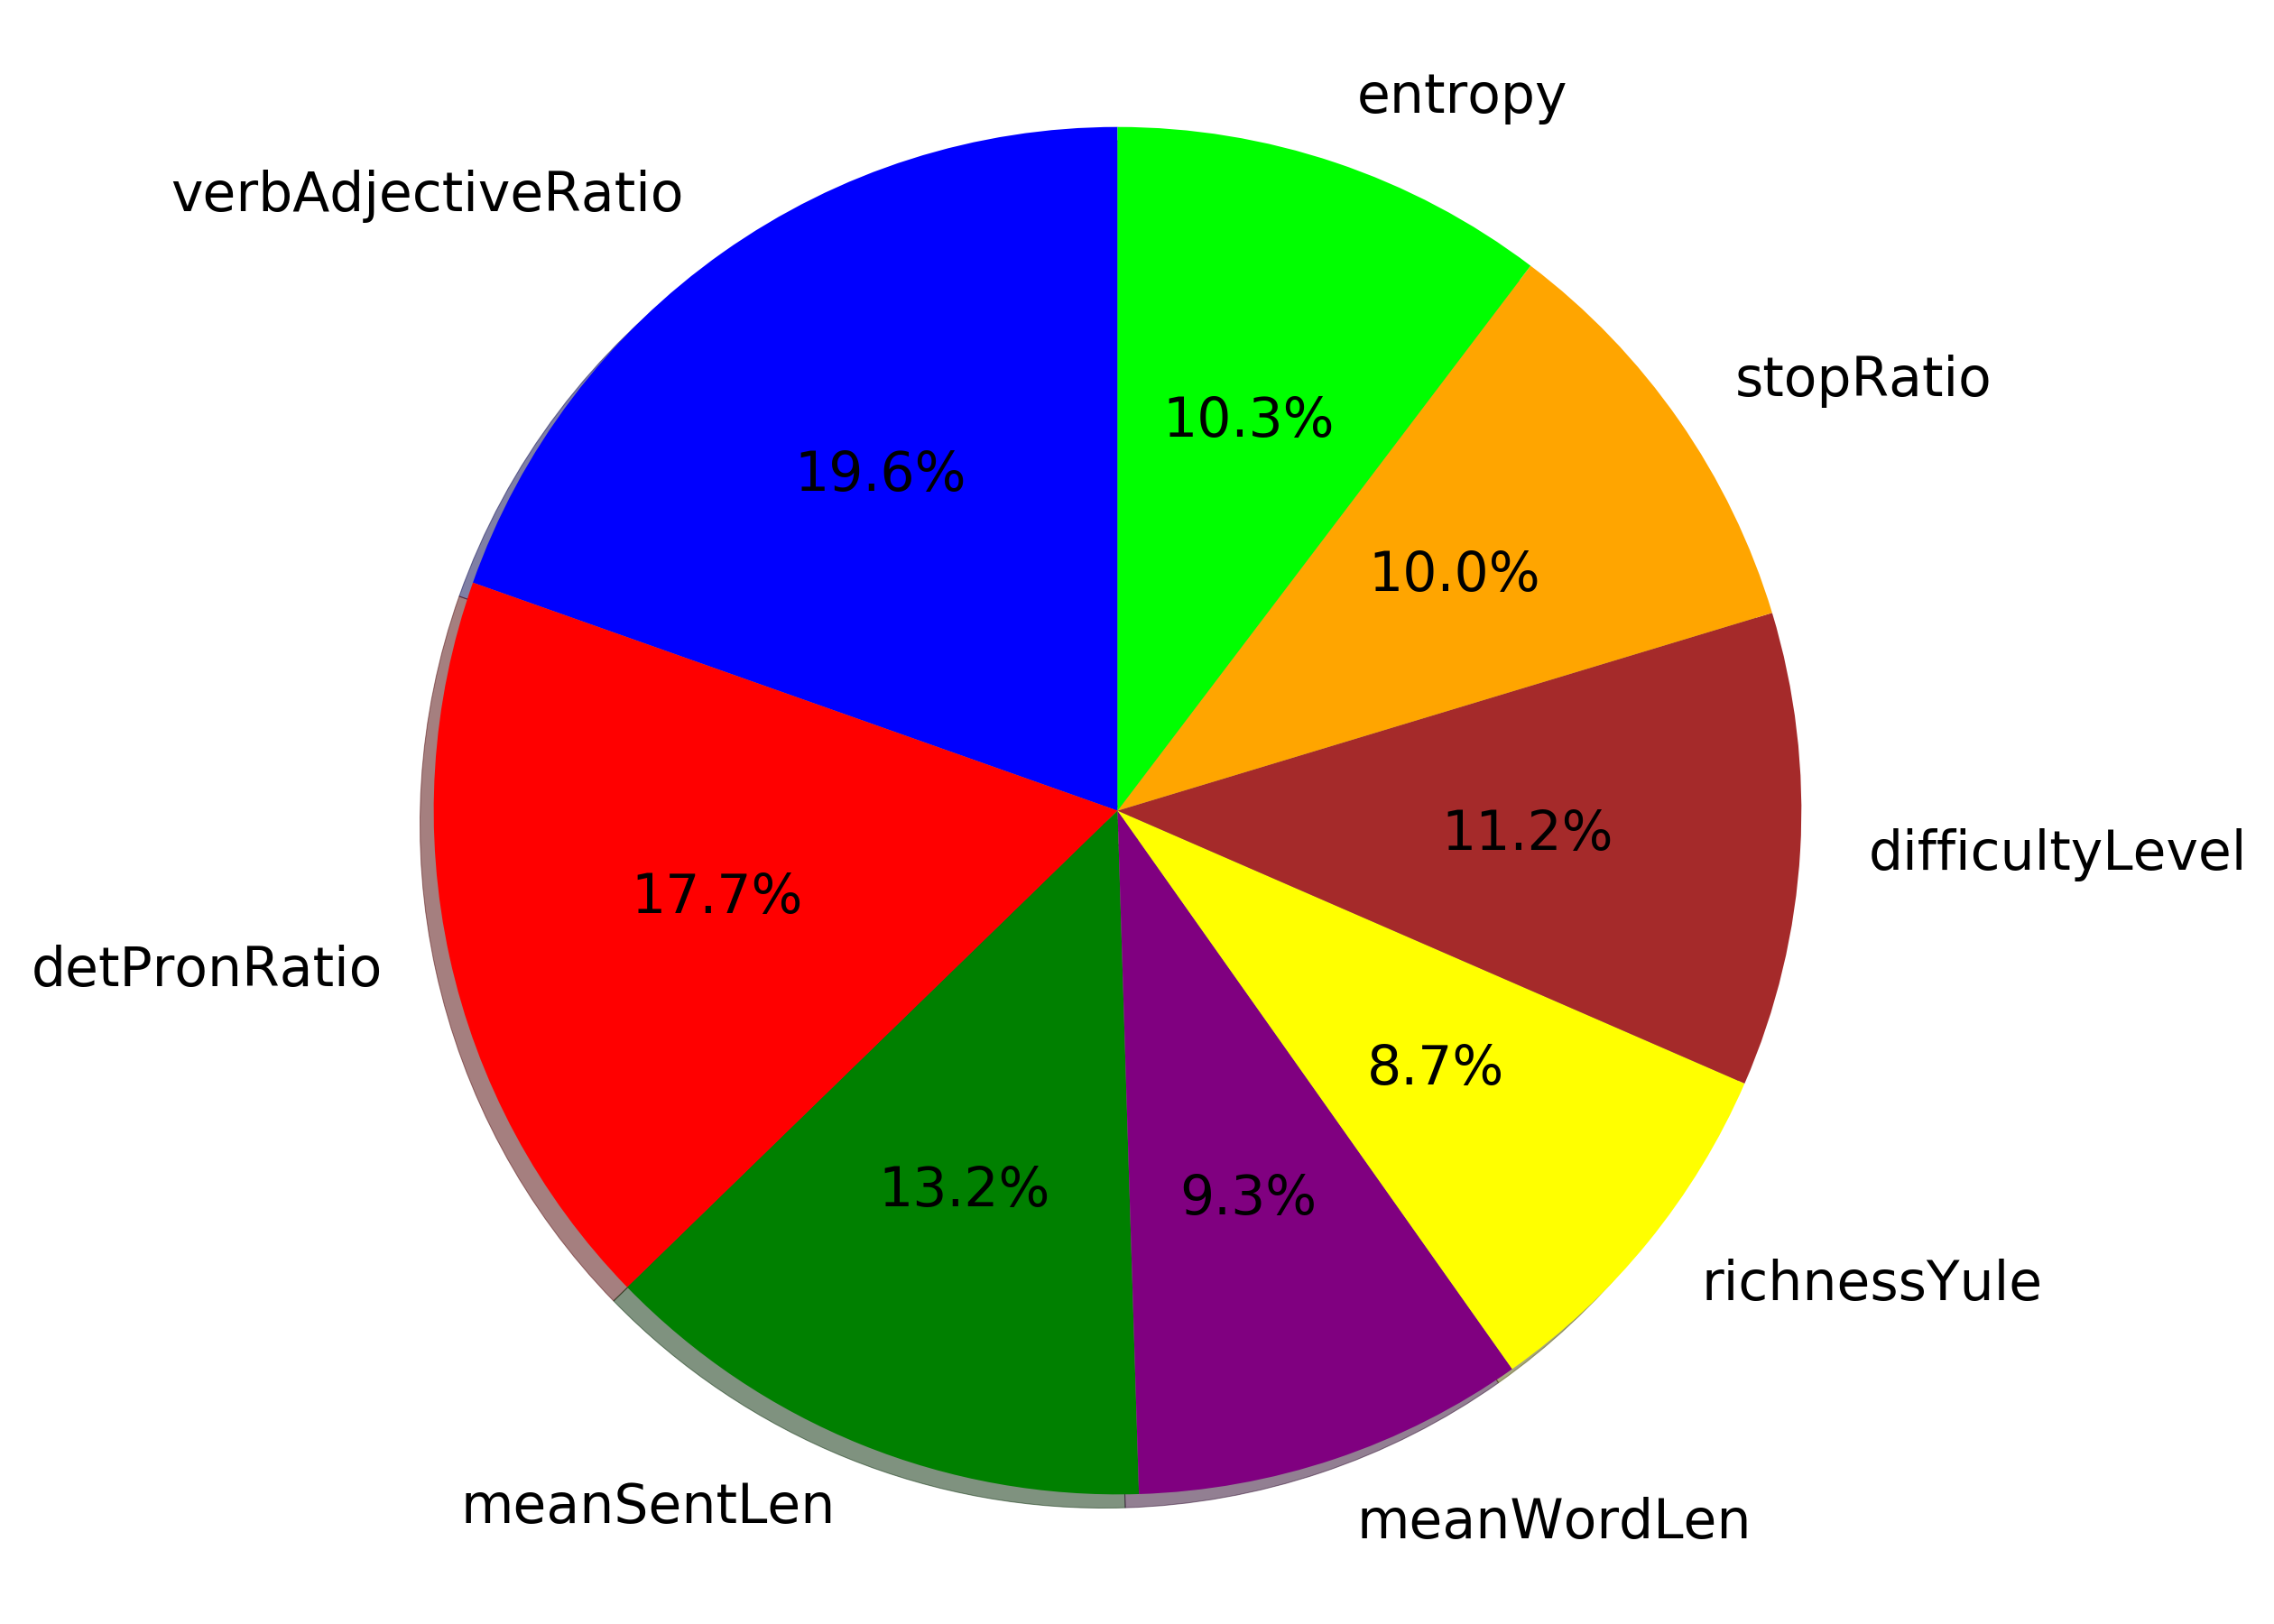
\includegraphics[width=0.8\textwidth]{Imagenes/Bitmap/DecisionTrees/pie8.png}}%
	\caption{Distribution of normalised feature importance with 8 features}%
	\label{fig:nfi8}
\end{figure}

In respect of the removed descriptors, some of them were deleted because they are related with another metric with has a bigger normalised feature importance. This is the case of \textit{ADJ}, \textit{VERB} (both related with \textit{verbAdjectiveRatio}), \textit{DET}, \textit{PRON} (this last two are related with \textit{detPronRatio}), \textit{numStopWords} (related with \textit{stopRatio}) and \textit{SimpsonIndex} (which is directly correlated with \textit{richnessYule}, due to their definitions). The unimportant style markers were also removed. In this case we have only two examples: \textit{numSemiColon} and \textit{num3Dots}.

On the other hand, we have deleted some style metrics due to their very low importance ratio and the existence of another style marker with a bigger value which is correlated with them. \textit{ADV}, \textit{ADP}, \textit{NOUN}, \textit{CONJ}, \textit{numCommas}, \textit{numDots}, \textit{numWords} and \textit{numDifWords} belong to this circumstances. The \textit{numBrackets} feature was removed only because of its extremely poor normalised feature importance (when it was deleted it had a value of 0.7\%).

We still have to explain the reasons why three style descriptors were eliminated. The \textit{depth} feature was removed because our purpose in this work is to develop a model which is based on the recipient of the message and not on its depth. Perhaps, it is possible to obtain characteristics of a message related to this style marker, for instance the length of the message, but this is not the goal of this work. The case of the elimination of \textit{richnessVocab} is due to its similarity to the \textit{richnessYule}, but less complexity and a very low normalised feature importance. Finally, we can also find similarities between \textit{charLenght} and \textit{meanSentLen} and \textit{meanWordLen}, which caused the first one to be eliminated.

In conclusion, thanks to the Gini Importance, we were able to measure how significant a metric is in conforming to the initially defined categorisation. This results from the nature of Decision Trees which are an easily explainable classification method. Hence we have selected eight different style markers which describes the writing style based on the recipient of the e-mail.